\lstset{
  language=SQL,                      % Chọn ngôn ngữ SQL
  basicstyle=\ttfamily\footnotesize, % Font không chân và nhỏ gọn
  keywordstyle=\color{blue},         % Màu xanh cho từ khóa
  stringstyle=\color{red},           % Màu đỏ cho chuỗi ký tự
  frame=single,                      % Viền đơn quanh đoạn mã
  extendedchars=true,                % Hỗ trợ ký tự đặc biệt
}

\begin{enumerate}[label=\alph*.]

    \item Tạo cơ sở dữ liệu:
    
    \begin{lstlisting}
    CREATE DATABASE IF NOT EXISTS bank_db;
    \end{lstlisting}
    
    \noindent{\textbullet\ Bảng branches:}
        
    \begin{lstlisting}
    CREATE TABLE IF NOT EXISTS bank_db.branches (
        branchCode VARCHAR(50)  NOT NULL 
            PRIMARY KEY,
        branchName VARCHAR(256) NOT NULL,
        province   VARCHAR(50)  NULL,
        district   VARCHAR(50)  NULL,
        street     VARCHAR(256) NULL
    );
    \end{lstlisting}

    \noindent{\textbullet\ Bảng customers:}
        
    \begin{lstlisting}
    CREATE TABLE IF NOT EXISTS bank_db.customers (
        customerID  VARCHAR(50)  NOT NULL 
            PRIMARY KEY,
        lastName    VARCHAR(50)  NOT NULL,
        firstName   VARCHAR(50)  NOT NULL,
        birthDate   DATE         NOT NULL,
        phoneNumber VARCHAR(15)  NULL,
        address     VARCHAR(256) NULL,
        creditScore INT          NULL
    );
    \end{lstlisting}

    \newpage

    \noindent{\textbullet\ Bảng employees:}
        
    \begin{lstlisting}
    CREATE TABLE IF NOT EXISTS bank_db.employees (
        employeeCode VARCHAR(50)  NOT NULL 
            PRIMARY KEY,
        lastName     VARCHAR(50)  NOT NULL,
        firstName    VARCHAR(50)  NOT NULL,
        position     VARCHAR(256) NULL,
        department   VARCHAR(256) NULL,
        managerCode  VARCHAR(50)  NULL,
        branchCode   VARCHAR(50)  NULL
    );
    \end{lstlisting}

    \noindent{\textbullet\ Bảng products:}
        
    \begin{lstlisting}
    CREATE TABLE IF NOT EXISTS bank_db.products (
        productCode  VARCHAR(50)  NOT NULL 
            PRIMARY KEY,
        productType  VARCHAR(256) NULL,
        interestRate FLOAT        NULL,
        term         INT          NULL,
        minAmount    BIGINT       NULL,
        maxAmount    BIGINT       NULL
    );
    \end{lstlisting}

    \noindent{\textbullet\ Bảng accounts:}
        
    \begin{lstlisting}
    CREATE TABLE IF NOT EXISTS bank_db.accounts (
        accountNumber VARCHAR(256) NOT NULL 
            PRIMARY KEY,
        accountName   VARCHAR(256) NOT NULL,
        balance       BIGINT       NOT NULL,
        customerID    VARCHAR(50)  NULL,
        productCode   VARCHAR(256) NULL,
        openingBranch VARCHAR(50)  NULL,
        openingDate   DATETIME DEFAULT (NOW()) NULL
    );
    \end{lstlisting}

    \noindent{\textbullet\ Bảng transactions:}
        
    \begin{lstlisting}
    CREATE TABLE IF NOT EXISTS bank_db.transactions (
        transactionNumber INT AUTO_INCREMENT
            PRIMARY KEY,
        sourceAccount     VARCHAR(50)  NULL,
        targetAccount     VARCHAR(50)  NULL,
        transactionType   VARCHAR(50)  NULL,
        amount            BIGINT       NOT NULL,
        time              DATETIME DEFAULT 
            CURRENT_TIMESTAMP NOT NULL,
        description       VARCHAR(256) NULL,
        employeeCode      VARCHAR(50)  NULL
    );
    \end{lstlisting}
        
    \newpage

    \noindent{\textbullet\ Tạo các ràng buộc dữ liệu:}

    \begin{lstlisting}
    ALTER TABLE bank_db.employees
        ADD CONSTRAINT branch___fk
            FOREIGN KEY (branchCode) 
            REFERENCES bank_db.branches (branchCode),
        ADD CONSTRAINT employees_managers__fk
            FOREIGN KEY (managerCode) 
            REFERENCES bank_db.employees (employeeCode);

    ALTER TABLE bank_db.accounts
        ADD CONSTRAINT customerID___fk
            FOREIGN KEY (customerID) 
            REFERENCES bank_db.customers (customerID),
        ADD CONSTRAINT openingBranch___fk
            FOREIGN KEY (openingBranch) 
            REFERENCES bank_db.branches (branchCode),
        ADD CONSTRAINT productCode___fk
            FOREIGN KEY (productCode) 
            REFERENCES bank_db.products (productCode);

    ALTER TABLE bank_db.transactions
        ADD CONSTRAINT sourceAccount___fk
            FOREIGN KEY (sourceAccount) 
            REFERENCES bank_db.accounts (accountNumber),
        ADD CONSTRAINT targetAccount___fk
            FOREIGN KEY (targetAccount) 
            REFERENCES bank_db.accounts (accountNumber),
        ADD CONSTRAINT transactions__fk
            FOREIGN KEY (employeeCode) 
            REFERENCES bank_db.employees (employeeCode);
    \end{lstlisting}

    \item Chèn dữ liệu

    % \begin{figure}[H]
    %     %\centering
    %     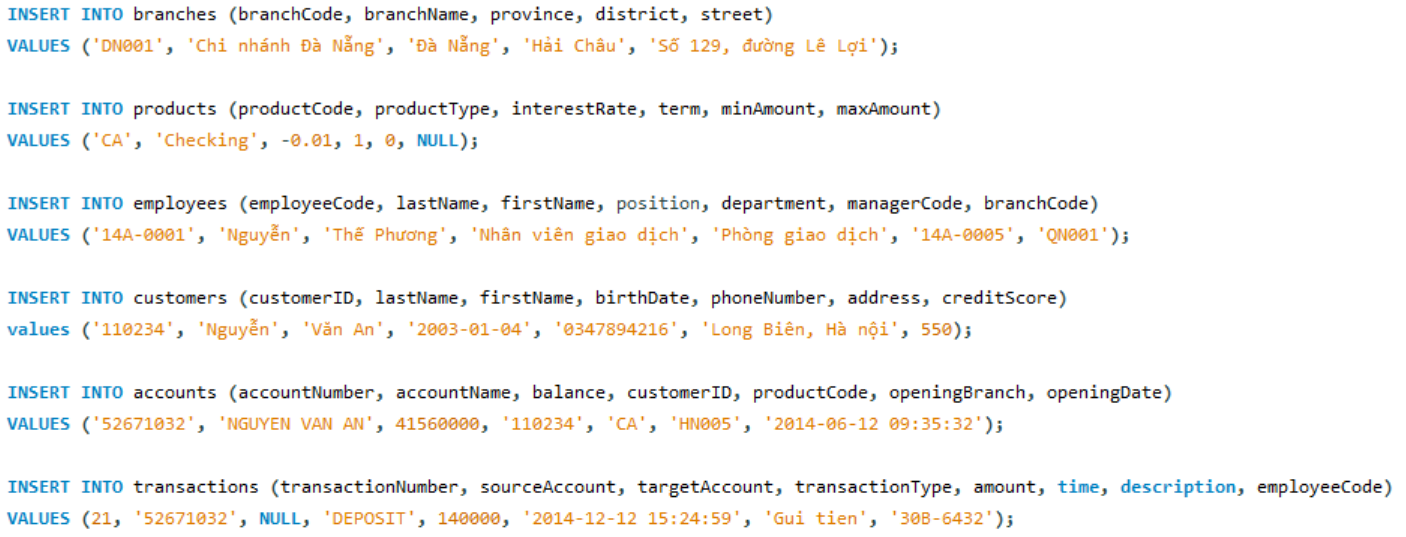
\includegraphics[width=\textwidth]{sample-insert.png}
    %     \caption{Một số ví dụ chèn dữ liệu vào các bảng.}
    %     \label{fig:sql-insert}
    % \end{figure}

    \begin{lstlisting}
    INSERT INTO branches
    (branchCode, branchName, province, district, street)
    VALUES
    ('DN001', 'Chi nhánh Đà Nẵng', 'Đà Nẵng', 'Hải Châu', 'Số 129, đường Lê Lợi');

    INSERT INTO products
    (productCode, productType, interestRate, term, minAmount, maxAmount)
    VALUES 
    ('CA', 'Checking', -0.01, 1, 0, NULL);

    INSERT INTO employees
    (employeeCode, lastName, firstName, position, department, managerCode, branchCode)
    VALUES 
    ('14A-0001', 'Nguyễn', 'Thế Phương', 'Nhân viên giao dịch', 'Phòng giao dịch', '14A-0005', 'QN001');

    INSERT INTO customers
    (customerID, lastName, firstName, birthDate, phoneNumber, address, creditScore)
    VALUES
    ('110234', 'Nguyễn', 'Văn An', '2003-01-04', '0347894216', 'Long Biên, Hà nội', 550);

    INSERT INTO accounts
    (accountNumber, accountName, balance, customerID, productCode, openingBranch, openingDate)
    VALUES
    ('52671032', 'NGUYEN VAN AN', 41560000, '110234', 'CA', 'HN005', '2014-06-12 09:35:32');

    INSERT INTO transactions
    (transactionNumber, sourceAccount, targetAccount, transactionType, amount, time, description, employeeCode)
    VALUES
    (21, '52671032', NULL, 'DEPOSIT', 140000, '2014-12-12 15:24:59', 'Gui tien', '30B-6432');
    \end{lstlisting}
 
\end{enumerate}
